\subsection{Class level}
	\subsubsection{Board}
	First the board is initialized, then the board has to initialize the controller. After that the board goes to the NOP state from which it can answer requests from robots and the controller. \\
Whenever a robot requests an invalid move via the moveRequest() function, the board sends out a moveRequest() == FAILED message and returns to the NOP state. But when a robot requests a correct move, the new position is calculated and stored using the functions calcuateNewLocation() and saveLocation(). \\
Normally the board now goes to the RequestedRobotMoved state from which it will send a hint if the robot stept on a hinttile, the board will always notify the controller that the board has been updated via the Controller.notifyViewer() function.\\
If the requested move would mean that other robots will get moved the board goes to the RequestedRobotMoved state with the Controller.notifyAutoMovement() function which means that the other robot will receive a notifyAutoMovement to let him know that he has been moved, all the other functions called are the same as with the regular move.\\
When a robot moves to it's homeTile, the boardResponse will be WIN and the game ends, then the board goes to the Game\_Over state and it can terminate or start a new game.\\
Every time a robot has made a move, the controller requests a tile-exchange via the requestTilesExchange() function, this exchange is performed by the board.\\
	
	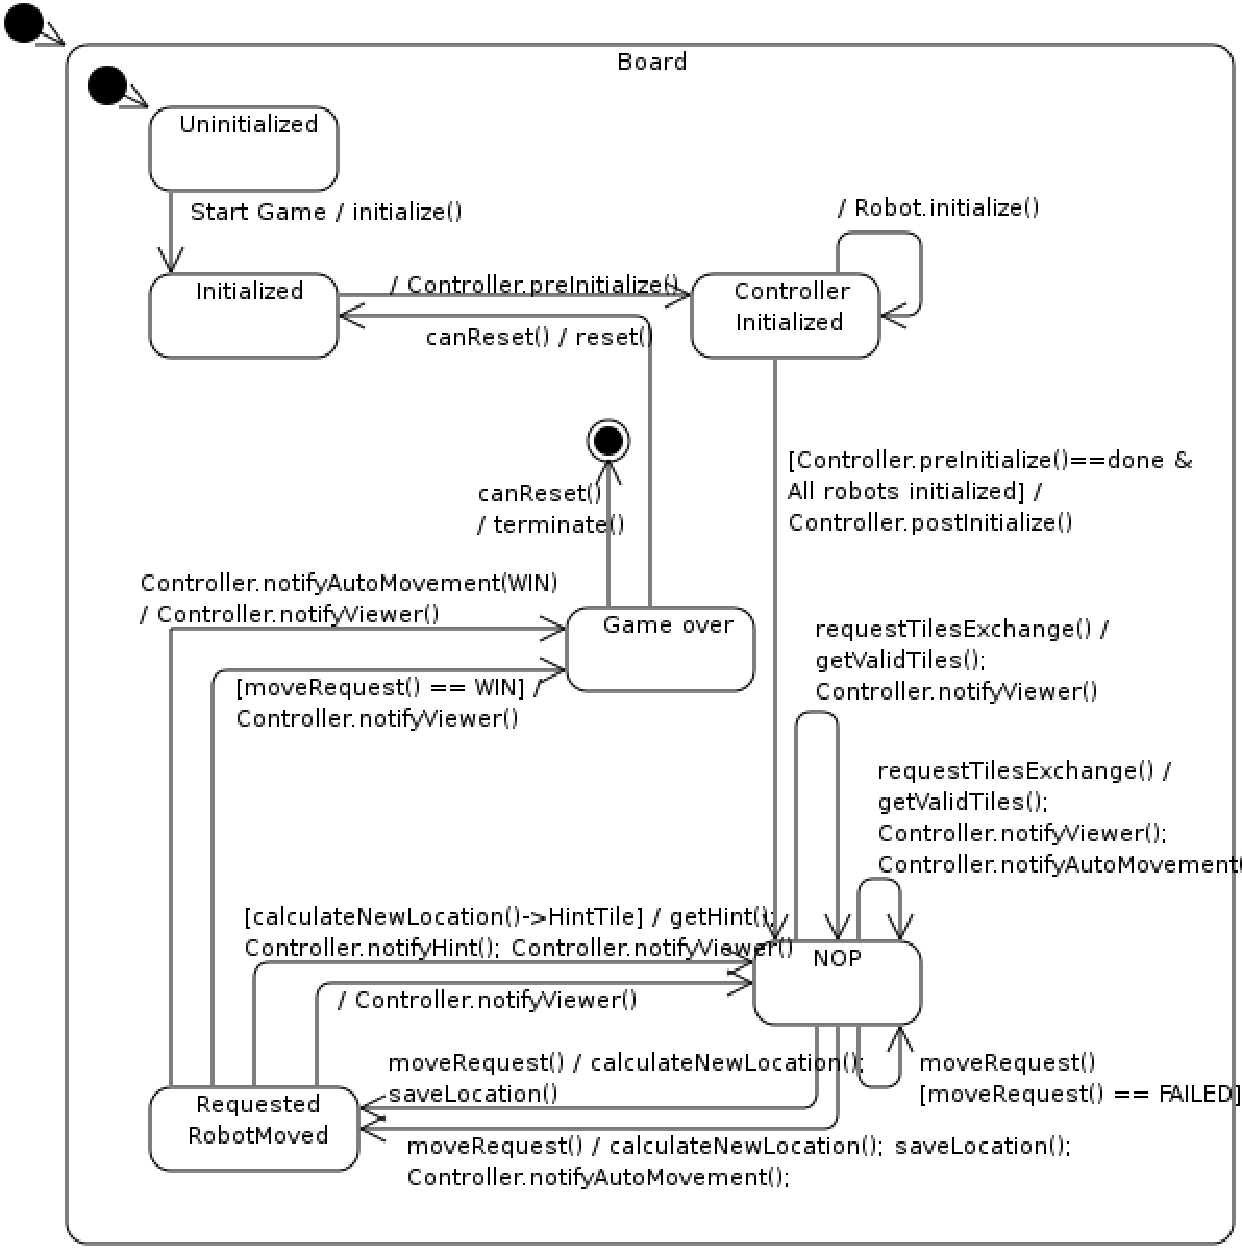
\includegraphics[width=\linewidth]{statecharts/board.pdf}

	\subsubsection{Controller}
	The controller initializes in two phases, the first phase is the preInitialize() during which it waits for other classes to initialize. The second phase is the postInitialize() function, when the controller is in this phase, it knows that all the other classes have been initialized and is aware of the state of all the classes and goes to the NOP state from which most actions take place.\\
If a robot requests a move, the controller goes in to the MoveRequested state, after that it goes to a new state depending on the response of the board. If the board response equals FAILED, the robot is not moved and the controller goes back to the NOP state. If the board response equals WIN the controller will send a notifyStateChange() and notifyGameOver() to let it know that the board has changed and the game has ended, it will also send a terminate() function to the other classes because the game is over and terminate itself in the end. If the board response equals SUCCES the controller switches 2 tiles using Board.requestTilesExchange() and sends a Robot.notifyHint() if needed, it will go to the TilesSwitched state and call the Viewer.notifyStateChange() either way.\\
After the 2 tiles are switched the robots that have been moved by this tileswitch are notified via the Robot.notifyAutoMovement() and the viewer receives an update via the Viewer.notifyStateChange().\\


	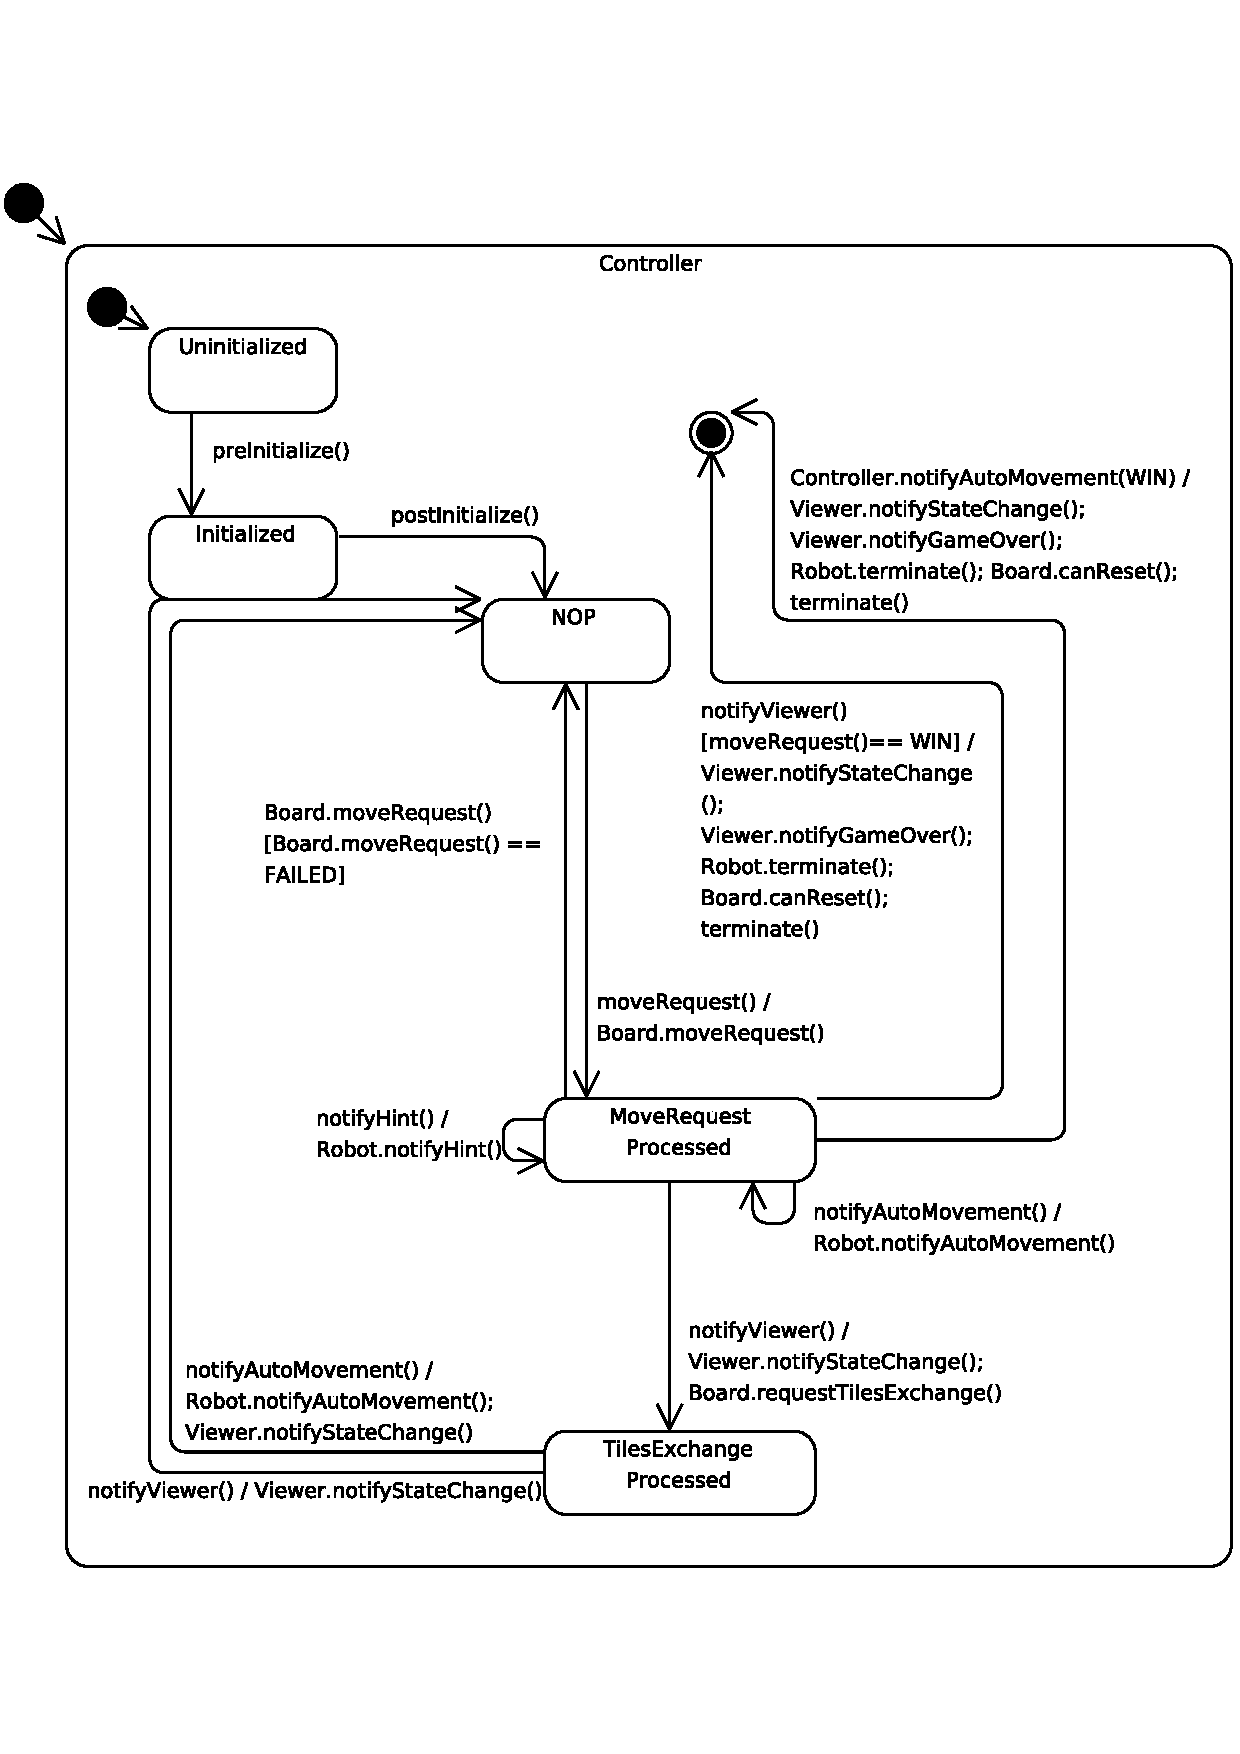
\includegraphics[width=\linewidth]{statecharts/controller.pdf}

	\subsubsection{Viewer}
	After being initialized the viewer comes in the NOP state, which means that it isn't doing anything, but it receives updates from the controller every now and then.... If the board has been changed the function updateView() is called to make the changes visible, it also sends out a notifyStateChange() to let the other classes know the state has changed. The viewer is removed when the game is over, but because there can be multiple viewers, it can also decide to remove itself.
	
	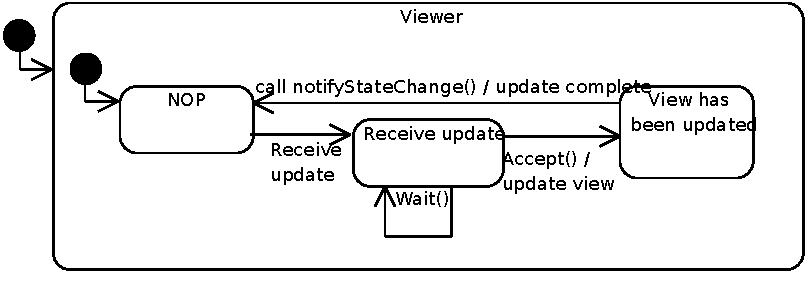
\includegraphics[width=\linewidth]{statecharts/view.pdf}

	\subsubsection{Robot}
	The robot class gets initialized by the controller, it starts at a randomly picked spot, which can be a normal tile, a hint tile or a conveyer tile. The robot receives a notifyAutomovement() every time it gets moved, this can happen in two ways: the robot steps on a conveyer belt or the robot gets moved via a tileswitch. Whenever a robot is on a tile It can request a move which can result in three ways: success, failed or win. If a move request is a success, the move is made, if a move request is a failure, the move is not made because the desired path of the moved Is blocked, if a move request results in a win it means that the robot has reached its hometile the game ends and this robot has won. When another robot wins this robot gets a terminate request from the controller and the game is over. The robot can also encounter hint tiles which point the robot to the location of its hometile.
	
	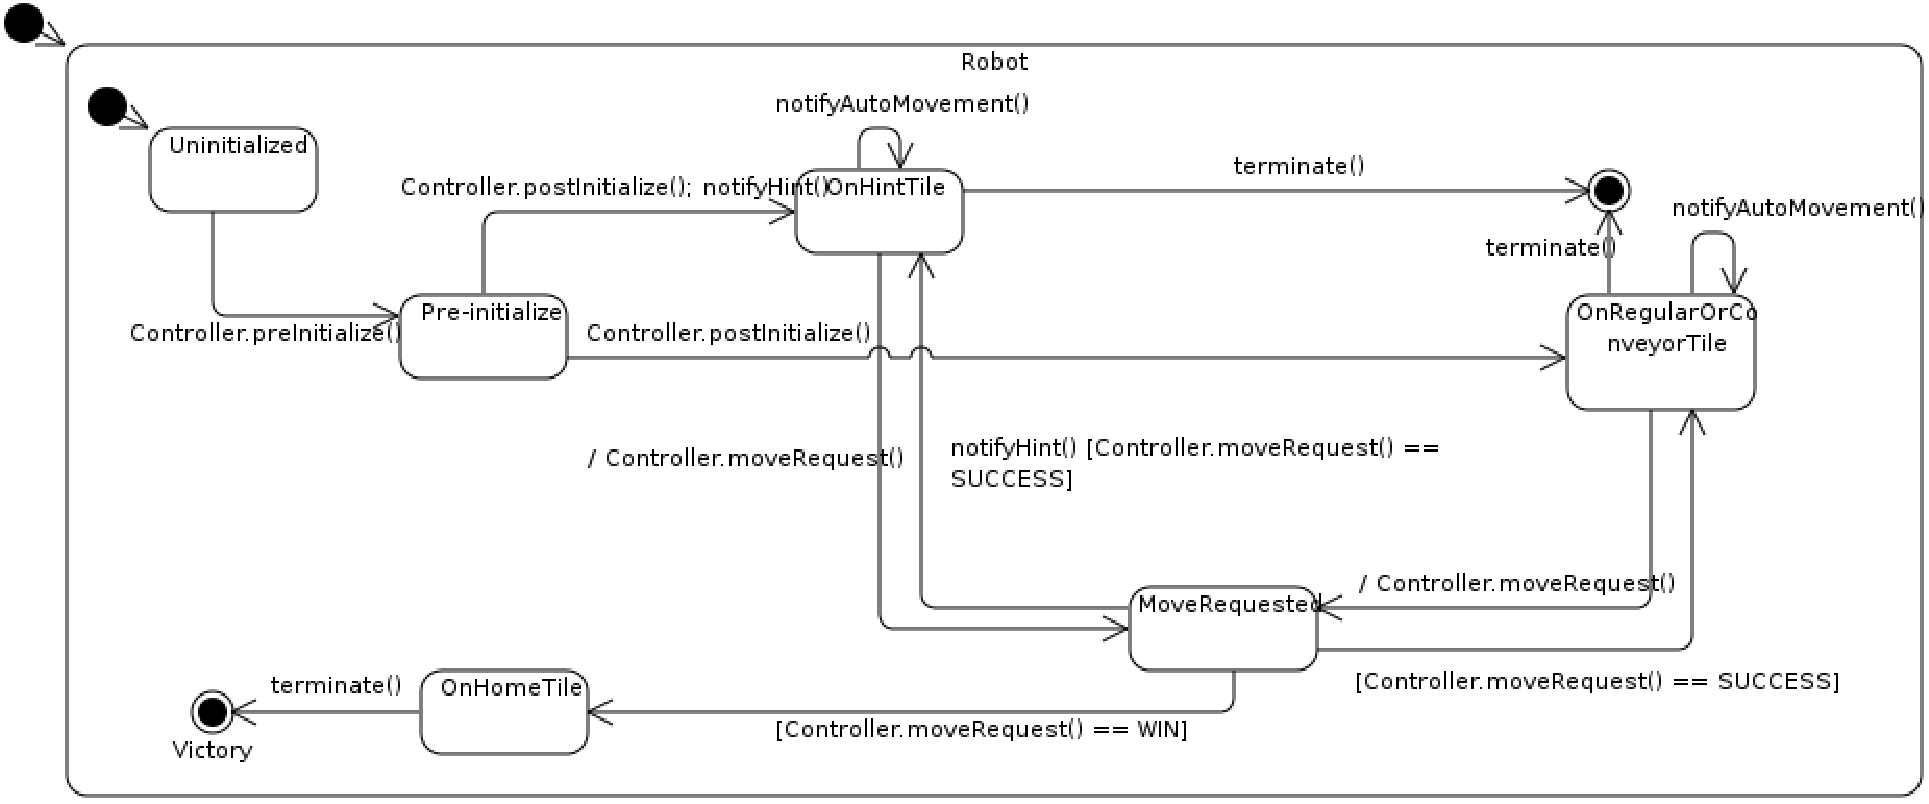
\includegraphics[width=\linewidth]{statecharts/robot.pdf}

\subsection{System level}
	The following graph is our system level state chart, which contains all our class level state charts and gives an overview of the complete system. Although this state chart is mostly trivial, it gives a more complete view of the entire system, thus it is shown below.

	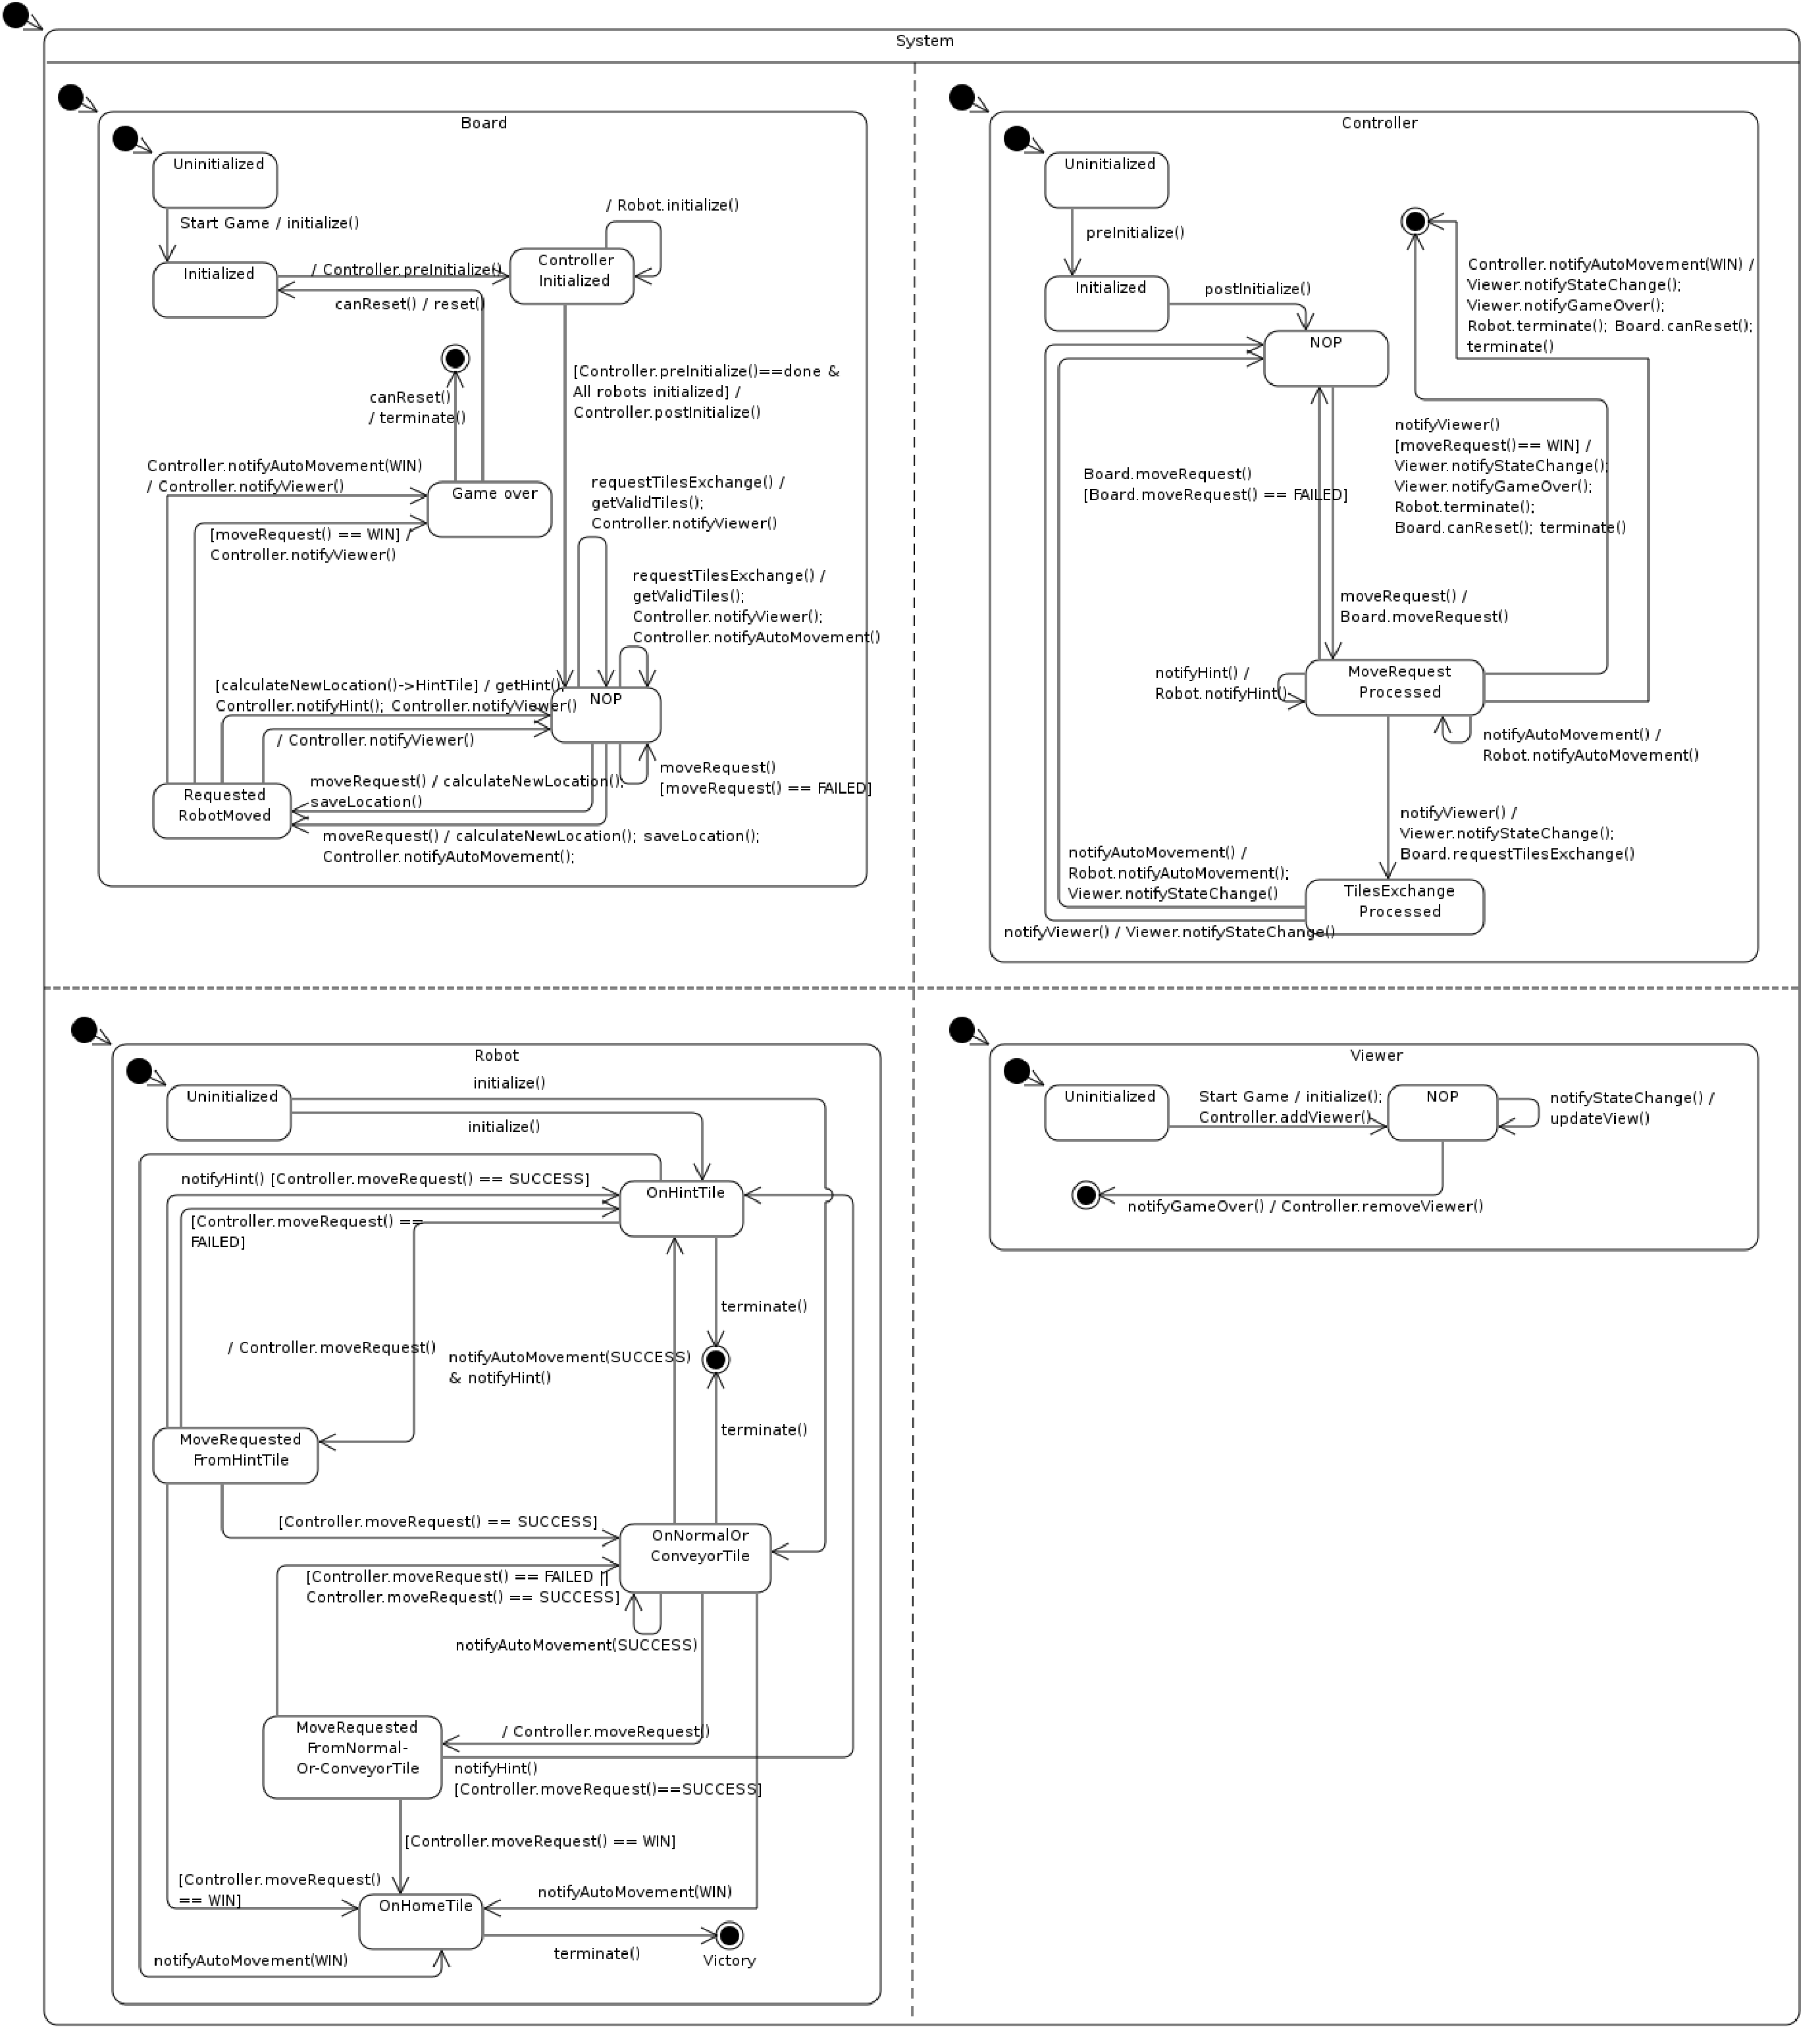
\includegraphics[width=\linewidth]{statecharts/system.pdf}

	
